\documentclass[12pt,a4paper]{article}

% ── Packages ─────────────────────────────────────────────────────────────────
\usepackage[utf8]{inputenc}
\usepackage{lmodern}
\usepackage[T1]{fontenc}
\usepackage[portuguese,english]{babel}
\usepackage{setspace}
\usepackage{tikz}
\usepackage{geometry}
\usepackage{graphicx}
\usepackage{booktabs}
\usepackage{multirow}
\usepackage{array}
\usepackage{amsmath}
\usepackage{listings}
\usepackage{xcolor}
\usepackage[hidelinks]{hyperref}
\usepackage{caption}
\usepackage{subcaption}
\usepackage{float}
\usepackage{siunitx}
\usepackage{pgfplots}
\usepackage{titlesec}
\usepackage{indentfirst}
\pgfplotsset{compat=1.18}

\geometry{
  top=2.5cm, bottom=2.5cm,
  left=2.5cm,  right=2.5cm
}

% ── Listing style ─────────────────────────────────────────────────────────────
\lstdefinestyle{cppstyle}{
  language=C++,
  basicstyle=\ttfamily\small,
  keywordstyle=\color{blue}\bfseries,
  commentstyle=\color{gray}\itshape,
  stringstyle=\color{orange},
  numbers=left,
  numberstyle=\tiny\color{gray},
  breaklines=true,
  frame=single,
  tabsize=4,
  showstringspaces=false,
}

\lstdefinestyle{ruststyle}{
  language=C,
  basicstyle=\ttfamily\small,
  keywordstyle=\color{blue}\bfseries,
  commentstyle=\color{gray}\itshape,
  stringstyle=\color{orange},
  numbers=left,
  numberstyle=\tiny\color{gray},
  breaklines=true,
  frame=single,
  tabsize=4,
  showstringspaces=false,
  morekeywords={fn,let,mut,usize,for,in,unsafe,use,pub,mod,impl,struct,enum,match,if,else,loop,break,return,vec,Vec,println,print},
}

\hypersetup{
    colorlinks=true,
    linkcolor=black,
    urlcolor=blue,
}

% ── Document ──────────────────────────────────────────────────────────────────
\begin{document}

% ── Custom cover page ─────────────────────────────────────────────────────────
\begin{titlepage}
\selectlanguage{portuguese}
\newgeometry{top=2cm, bottom=2cm, left=2.5cm, right=2.5cm}

\vspace*{0.3cm}
\begin{center}

  % Logo + institution block
  
\includegraphics[height=2.2cm]{feup-logo}
  \hspace{0.5cm}
  \begin{minipage}[b]{0.6\textwidth}
    \raggedright
    {\large\bfseries Faculdade de Engenharia}\\[0.1em]
    {\large\bfseries da Universidade do Porto}\\[0.4em]
    {\normalsize Licenciatura em Engenharia}\\
    {\normalsize Informática e Computação (L.EIC)}
  \end{minipage}

  \vspace{1.2cm}
  \noindent\rule{\linewidth}{1.2pt}
  \vspace{0.4cm}

  {\large Computação Paralela e Distribuída (CPD)}\\[0.15em]
  {\normalsize Turma T07 \textbullet{} Grupo 13 \textbullet{} 2025/2026}

  \vspace{0.4cm}
  \noindent\rule{\linewidth}{1.2pt}

  \vspace{2.5cm}
  {\LARGE Performance Evaluation of}\\[0.5em]
  {\LARGE Matrix Multiplication}\\[0.7em]
  {\large\itshape Single-Core and Multi-Core Performance Analysis}

  \vspace{3cm}

  {\normalsize
  \begin{tabular}{l l}
    \textbf{André Pinho}           & \texttt{up202307008} \\[0.3em]
    \textbf{Duarte Martins}        & \texttt{up202304549} \\[0.3em]
    \textbf{Maria Beatriz Leite}   & \texttt{up202307229} \\
  \end{tabular}}

  \vfill

  {\normalsize Porto, March 2026}

\end{center}
\restoregeometry
\selectlanguage{english}
\end{titlepage}
\clearpage

\tableofcontents
\clearpage

\listoffigures
\clearpage

\listoftables
\clearpage

% ─────────────────────────────────────────────────────────────────────────────
\section{Introduction}
\label{sec:intro}
% ─────────────────────────────────────────────────────────────────────────────

\begin{center}
\textit{``Bad programmers worry about the code. Good programmers worry about
data structures and their relationships.''} --- Linus Torvalds
\end{center}

\medskip

The goal of this report is to investigate how the memory hierarchy affects
processor performance when accessing large amounts of data, and how this
impacts both single-core and multi-core CPU performance.

To that end, we chose matrix multiplication as our primary computational
workload and divided the study into two parts, conducting separate
investigations on single-core and multi-core performance respectively.

For the single-core evaluation, we designed three distinct algorithms to
multiply two $n \times n$ matrices and measured their performance against one
another:

\begin{enumerate}
  \item \textbf{Generic Multiplication} -- The naive, textbook implementation
        of matrix multiplication. It iterates over rows and columns in the
        natural mathematical order, offering no optimisations for memory access
        patterns, making it a useful baseline for comparison.
  \item \textbf{Line Multiplication} -- A reformulation of the access order to
        improve spatial locality. By reordering the loop traversal to access
        memory more sequentially, this algorithm reduces cache misses compared
        to the generic approach.
  \item \textbf{Block-Oriented Multiplication} -- A cache-aware algorithm that
        divides the matrices into smaller sub-blocks sized to fit within the
        cache. By operating on these blocks, it maximises data reuse and
        significantly reduces the cost of memory access for large matrices.
\end{enumerate}

All three algorithms share the same computational complexity of $2n^3$
floating-point operations for an $n \times n$ matrix, so any difference in
throughput is purely a consequence of memory access behaviour. Performance is
expressed in GFlop/s:

\begin{equation}
  \text{Performance (GFlop/s)} = \frac{2n^3}{T \times 10^9}
  \label{eq:gflops}
\end{equation}

\noindent where $T$ is the wall-clock execution time in seconds.

After benchmarking all three algorithms in C++, we extended the comparison to
Rust, allowing us to evaluate not only the relative performance of the
algorithms themselves, but also the native performance characteristics of each
language.

The second part of the report scales the analysis to a multi-core
architecture. We implemented parallel versions of the first and second
algorithms using OpenMP, and tested them across varying matrix sizes and thread
counts, measuring key metrics including GFlop/s, speedup, and efficiency.

Taken together, this report presents graphical representations of the
performance achieved across all experiments. By comparing execution times,
cache behaviour, and parallelisation strategies, we draw concrete conclusions
regarding the most effective methods for optimising computational throughput.

% ─────────────────────────────────────────────────────────────────────────────
\subsection{Why Rust?}
\label{sec:why-rust}
% ─────────────────────────────────────────────────────────────────────────────

The project invited us to choose a programming language of our liking and
compare the performance of different matrix multiplication algorithms across
C++ and that chosen language. Our choice was Rust. Beyond being an opportunity
to explore a language that had remained unexplored throughout the course, it
also sparked curiosity regarding the claim that \textit{``Rust is faster than
C++.''}\ However, ``fast'' is a broad term when comparing programming
languages --- a language can excel in memory access and management while
falling behind in other areas, such as graph traversal.

In light of this project, we decided to put that claim to the test and verify
whether Rust is, in fact, faster than C++ for single-core matrix
multiplication.

For a fair comparison, we evaluated both variants of Rust: \textit{safe Rust}
and \textit{unsafe Rust}. The former enforces memory safety at compile time
through a system of ownership, borrowing, and lifetime rules, and additionally
performs bounds checking on array and slice accesses at runtime.
\textit{Unsafe Rust}, as the name implies, lowers those guardrails and places
memory management in the hands of the programmer. Crucially, it also allows
bounds checking to be bypassed, and we expect this reduction in runtime
overhead to have a measurable impact on performance when benchmarking both
variants.

As for our predictions, we believe the most performant language will be C++,
given its decades of tooling and optimisation, and its status as the
established leader in systems programming --- particularly in
high-performance, memory-intensive workloads. Since C++ also performs no
bounds checking by default, we expect \textit{unsafe Rust} to perform
comparably, though we still place C++ marginally ahead. \textit{Safe Rust},
carrying the cost of runtime bounds checks, is expected to come in last.

% ─────────────────────────────────────────────────────────────────────────────
\subsection{OpenMP: Parallelism vs.\ SIMD}
\label{sec:openmp-parallelism-vs-simd}
% ─────────────────────────────────────────────────────────────────────────────

To understand the second part of the performance evaluation, it is useful to
clarify what threads and cores are. A thread, in the programming
sense, is the smallest sequence of programmed instructions that can be managed
independently by a scheduler. As a simple illustration: if a program requires
50 independent iterations to produce a result, distributing that work across 5
threads assigns roughly 10 iterations to each, reducing the total execution
time by a factor of approximately 5 --- a $5\times$ speedup. In practice,
thread management introduces its own overhead, but the principle holds. A
core is an independent processing unit within a CPU that fetches and
executes instructions; a modern CPU contains multiple cores, each capable of
running one or more threads concurrently.

The second part of this evaluation compares the performance of single-core and
multi-core execution on the same matrix multiplication workloads.

To carry this out, we relied on the OpenMP library in C++, making use of two
directives:

\begin{itemize}
  \item \texttt{\#pragma omp parallel for} --- This directive spawns a team of
        threads and distributes the loop's iterations among them, enabling
        true multi-core parallelism. It is well-suited to computationally
        demanding, independent workloads, but introduces overhead from thread
        creation and synchronisation, which can hurt performance on simple or
        short-running loops.

  \item \texttt{\#pragma omp simd} --- Rather than distributing work across
        multiple threads, this directive instructs the compiler to vectorise
        the loop using SIMD (Single Instruction, Multiple Data) CPU
        instructions. This allows the processor to operate on multiple data
        elements in a single instruction cycle, improving throughput while
        remaining entirely single-core. It works best on tight, memory-dense
        loops over contiguous arrays, but requires that the data layout
        supports vectorisation.
\end{itemize}

Both approaches have distinct strengths and limitations. Parallelism excels in
heavy, independent computations but requires thread safety --- each iteration
must be independent of the others to avoid race conditions. SIMD excels in
dense, regular memory access patterns but demands contiguous data and is
constrained by the vector width of the underlying hardware. Understanding when
to apply each is key to effective performance optimisation.

\section{Experimental Setup}
\label{sec:setup}

\subsection{Hardware}
\label{subsec:hw}

\begin{table}[H]
  \centering
  \caption{Hardware platform (university machines -- \texttt{feup-b204d04}).}
  \label{tab:hw}
  \begin{tabular}{ll}
    \toprule
    \textbf{Component} & \textbf{Specification} \\
    \midrule
    CPU Model         & Intel\textsuperscript{\textregistered} Core\texttrademark{} i7-14700T (Raptor Lake) \\
    P-core / E-core   & 8P + 12E = 20 physical cores, 28 threads \\
    P-core Turbo      & up to 5.2~GHz \\
    L1 Data Cache     & 48~KB per P-core / 32~KB per E-core \\
    L2 Cache          & 2~MB per P-core / 2~MB per 4 E-cores \\
    L3 Cache          & 33~MB shared \\
    RAM               & 32~GiB DDR5 \\
    OS / Kernel       & Ubuntu 24.04.3 LTS / Linux 6.17.0-14-generic \\
    \bottomrule
  \end{tabular}
\end{table}

% ─────────────────────────────────────────────────────────────────────────────
\subsection{Software, Compilation \& Measurement Methodology}
\label{subsec:software-compilation-methodology}
% ─────────────────────────────────────────────────────────────────────────────

For the first experiment, C++ was compiled with GCC: \texttt{g++ -O2} for the
Generic algorithm, and \texttt{g++ -O3 -fno-plt -flto -march=native} for the
Line and Block variants, enabling auto-vectorisation and link-time
optimisation. Rust was compiled with \texttt{cargo build --release}
(edition 2024); the unsafe variant uses \texttt{get\_unchecked} to elide
bounds checks.

Execution time was measured using POSIX \texttt{clock()} in C++ and
\texttt{std::time::Instant} in Rust. Hardware performance counters were
collected via Linux \texttt{perf}:

\begin{verbatim}
perf stat -e cpu_core/mem_load_retired.l1_miss/,\
           cpu_core/mem_load_retired.l2_miss/ \
           ./bin/<executable>
\end{verbatim}

For the second experiment, the POSIX \texttt{clock()} function could not be
reused, as it measures per-thread CPU time rather than wall-clock elapsed time.
In a multi-threaded programme, each thread accumulates its own CPU time
independently, so sampling \texttt{clock()} yields the total CPU time consumed
across all threads combined --- not the actual duration of the parallel region
as observed by the user. To obtain a meaningful wall-clock measurement, timing
was instead performed using OpenMP's \texttt{omp\_get\_wtime()}, which returns
elapsed real time from a fixed reference point and is consistent across all
threads in the team.

For both experiments, each matrix is filled with non-null values prior to
multiplication.

% ─────────────────────────────────────────────────────────────────────────────
\section{Single-Core Results and Discussion}
\label{sec:results}
% ─────────────────────────────────────────────────────────────────────────────

% ─────────────────────────────────────────────────────────────────────────────
\subsection{Basic Matrix Multiplication Algorithm -- \textit{BMMA}}
\label{subsec:res_basic}
% ─────────────────────────────────────────────────────────────────────────────

\begin{table}[H]
  \centering
  \caption{Execution time (s) and GFlop/s -- \textit{BMMA}.}
  \label{tab:time_basic}
  \sisetup{round-mode=places, round-precision=3}
  \begin{tabular}{
      S[table-format=4.0, round-precision=0]
      S[table-format=6.3]
      S[table-format=5.3]
      S[table-format=6.3]
      S[table-format=5.3]
      S[table-format=7.3]
      S[table-format=5.3]
    }
    \toprule
    & \multicolumn{2}{c}{\textbf{C++}} & \multicolumn{2}{c}{\textbf{Rust safe}} & \multicolumn{2}{c}{\textbf{Rust unsafe}} \\
    \cmidrule(lr){2-3}\cmidrule(lr){4-5}\cmidrule(lr){6-7}
    {Size ($n$)} & {Time (s)} & {GFlop/s} & {Time (s)} & {GFlop/s} & {Time (s)} & {GFlop/s} \\
    \midrule
    1024 &   2.269 & 0.947 &   2.411 & 0.892 &   2.440 & 0.881 \\
    1536 &   8.846 & 0.820 &   8.347 & 0.869 &   8.855 & 0.819 \\
    2048 &  32.691 & 0.526 &  32.628 & 0.527 &  30.716 & 0.560 \\
    2560 &  63.584 & 0.528 &  60.077 & 0.558 &  64.320 & 0.522 \\
    3072 & 135.961 & 0.427 & 144.294 & 0.402 & 191.735 & 0.303 \\
    \bottomrule
  \end{tabular}
\end{table}

\begin{figure}[H]
  \centering
  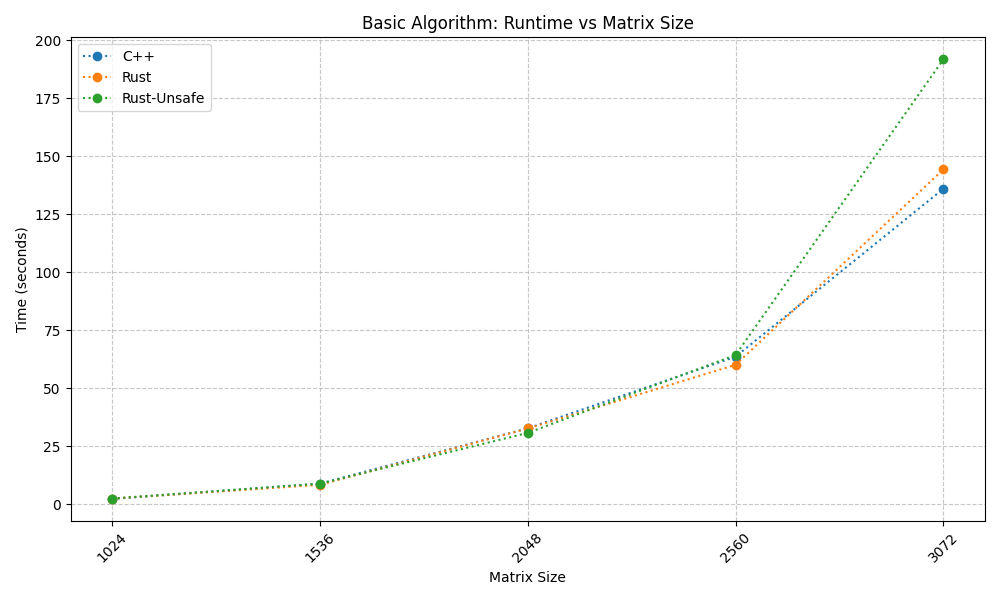
\includegraphics[width=0.85\linewidth]{../results/pythonGraphs/graphImgs/time_basic.png}
  \caption{Execution time (s) of the \textit{BMMA} for C++ and Rust variants.}
  \label{fig:time_basic}
\end{figure}

As expected, the linear growth of matrix size causes an exponential growth in
execution time, consistent with the $O(n^3)$ time complexity shared by all
three implementations (Table~\ref{tab:time_basic}, Figure~\ref{fig:time_basic}).

For smaller matrices, all three implementations perform nearly identically,
suggesting that at these scales memory access patterns and CPU pipeline
behaviour dominate over any language-level overhead. However, at $n = 3072$,
Rust unsafe degrades significantly, reaching $\sim$191\,s versus $\sim$136\,s
for C++ and $\sim$144\,s for Rust safe.

This did not align with our initial predictions, and we do not have a
definitive explanation for this behaviour. One hypothesis is that, given the
low algorithmic complexity of the \textit{BMMA}, the compiler retains enough
freedom in safe Rust to apply optimisations that the manually managed unsafe
variant inadvertently prevents. Another possibility is that our unsafe
implementation introduces a suboptimal memory access pattern that the compiler
cannot compensate for, whereas in safe Rust it retains full optimisation
freedom.

The GFlop/s drops consistently as matrix size increases across all three
implementations (Table~\ref{tab:time_basic}) --- from $\sim$0.9\,GFlop/s at $n = 1024$ down to
$\sim$0.3$-$0.5\,GFlop/s at $n = 3072$. This is a direct signature of cache
pressure: as the matrices grow, they no longer fit in the CPU cache and must
be stored in main memory (RAM), causing an increasing number of expensive
memory accesses. The CPU consequently spends the majority of its time idle,
waiting for data rather than performing floating-point operations.

In summary, our initial prediction --- C++ fastest, unsafe Rust second, safe
Rust last --- is not validated. The \textit{BMMA} is so memory-bound that
language-level differences are largely irrelevant, and any manual memory
management that disrupts the compiler's ability to auto-optimise can actively
hurt performance.

\begin{table}[H]
  \centering
  \caption{Absolute L1 and L2 cache misses (\texttt{perf}) -- \textit{BMMA},
           representative sizes.}
  \label{tab:perf_basic}
  \begin{tabular}{llrr}
    \toprule
    \textbf{Implementation} & \textbf{Size} & \textbf{L1 misses} & \textbf{L2 misses} \\
    \midrule
    C++         & 1024 & 977{,}005{,}348      & 964{,}652{,}322      \\
    Rust safe   & 1024 & 949{,}645{,}863      & 945{,}451{,}440      \\
    Rust unsafe & 1024 & 935{,}629{,}538      & 891{,}470{,}704      \\
    C++         & 3072 & 28{,}330{,}584{,}448 & 27{,}069{,}543{,}109 \\
    Rust safe   & 3072 & 28{,}965{,}326{,}258 & 26{,}691{,}467{,}818 \\
    Rust unsafe & 3072 & 28{,}700{,}870{,}188 & 27{,}180{,}702{,}512 \\
    \bottomrule
  \end{tabular}
\end{table}

The raw miss counts in Table~\ref{tab:perf_basic} can be misleading in
isolation: a larger absolute number of misses does not necessarily imply a
higher miss rate, since larger matrices also require exponentially more
operations. To enable a fair comparison across matrix sizes, the misses are
normalised as follows:

\begin{equation}
  \text{Normalised misses} = \frac{\text{L1 or L2 cache misses}}{n^3}
  \label{eq:norm_misses}
\end{equation}

\begin{figure}[H]
  \centering
  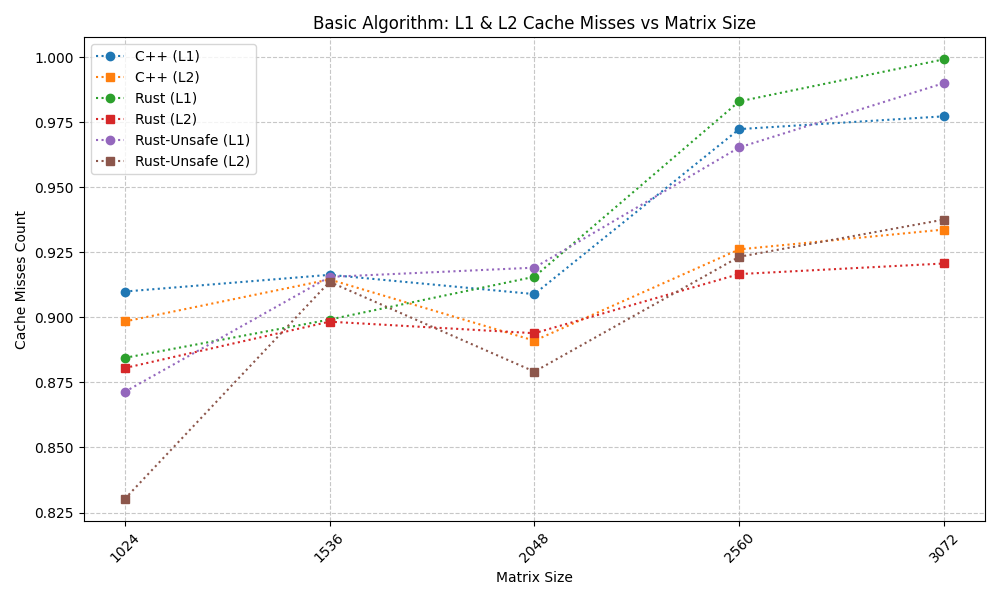
\includegraphics[width=0.85\linewidth]{../results/pythonGraphs/graphImgs/misses_basic.png}
  \caption{Normalised L1 and L2 cache misses of the \textit{BMMA} -- C++ and
           Rust variants.}
  \label{fig:misses_basic}
\end{figure}

After normalisation (Equation~\ref{eq:norm_misses}), the miss rates are extraordinarily high across the board,
with all implementations sitting between 0.83 and 1.00 at every matrix size
(Figure~\ref{fig:misses_basic}).
This means that for nearly every memory access, the requested data is absent
from cache --- confirming that the \textit{BMMA} is almost entirely
memory-bound, which directly explains the low and declining GFlop/s values.

As $n$ increases, the normalised miss rates trend upward for all
implementations, converging toward 1.0 at $n = 3072$. This is fully
consistent with the GFlop/s decline: larger matrices do not fit in cache, and
the naive access pattern --- which strides through the columns of the second
matrix --- makes no attempt to exploit spatial locality, so cache pressure
compounds rapidly with matrix size.

A visible dip in miss rates occurs at $n = 2048$, most notably for L2. This
is likely an artefact of cache set associativity alignment at that particular
matrix dimension, or it may reflect the boundary at which the matrices
transition between fitting partially and not at all within a given cache level.
It is worth noting, but should not be over-interpreted.

L2 miss rates are lower than L1 across all implementations, which is expected:
L2 catches a fraction of what L1 misses, and the gap between the two lines for
each implementation represents the fraction of misses serviced by L2 before
requiring a full trip to main memory.

In short, Figure~\ref{fig:misses_basic} provides the mechanistic explanation for the
runtime results in Table~\ref{tab:time_basic}: execution time grows and GFlop/s falls precisely because
normalised miss rates (Equation~\ref{eq:norm_misses}) are so high and increase with matrix size.

% ─────────────────────────────────────────────────────────────────────────────
\subsection{Line-by-Line Algorithm -- \textit{LLA}}
\label{subsec:res_line}
% ─────────────────────────────────────────────────────────────────────────────

\begin{table}[H]
  \centering
  \caption{Execution time (s) and GFlop/s -- \textit{LLA}.}
  \label{tab:time_line}
  \sisetup{round-mode=places, round-precision=3}
  \begin{tabular}{
      S[table-format=5.0, round-precision=0]
      S[table-format=6.3]
      S[table-format=6.3]
      S[table-format=7.3]
      S[table-format=6.3]
      S[table-format=7.3]
      S[table-format=6.3]
    }
    \toprule
    & \multicolumn{2}{c}{\textbf{C++}} & \multicolumn{2}{c}{\textbf{Rust safe}} & \multicolumn{2}{c}{\textbf{Rust unsafe}} \\
    \cmidrule(lr){2-3}\cmidrule(lr){4-5}\cmidrule(lr){6-7}
    {Size ($n$)} & {Time (s)} & {GFlop/s} & {Time (s)} & {GFlop/s} & {Time (s)} & {GFlop/s} \\
    \midrule
    1024  &    0.129 & 16.638 &    0.638 &  3.362 &    0.329 &  6.521 \\
    1536  &    0.433 & 16.724 &    2.205 &  3.284 &    1.093 &  6.626 \\
    2048  &    1.525 & 11.263 &    5.400 &  3.179 &    2.945 &  5.830 \\
    2560  &    3.762 &  8.921 &   10.876 &  3.085 &    7.017 &  4.785 \\
    3072  &    7.196 &  8.058 &   19.395 &  2.990 &   11.184 &  5.185 \\
    4096  &   19.127 &  7.186 &   47.484 &  2.896 &   28.252 &  4.868 \\
    6144  &   68.678 &  6.752 &  161.068 &  2.879 &   96.758 &  4.795 \\
    8192  &  167.392 &  6.572 &  393.142 &  2.799 &  230.160 &  4.783 \\
    10240 &  323.029 &  6.646 &  755.689 &  2.841 &  449.949 &  4.772 \\
    \bottomrule
  \end{tabular}
\end{table}

\begin{figure}[H]
  \centering
  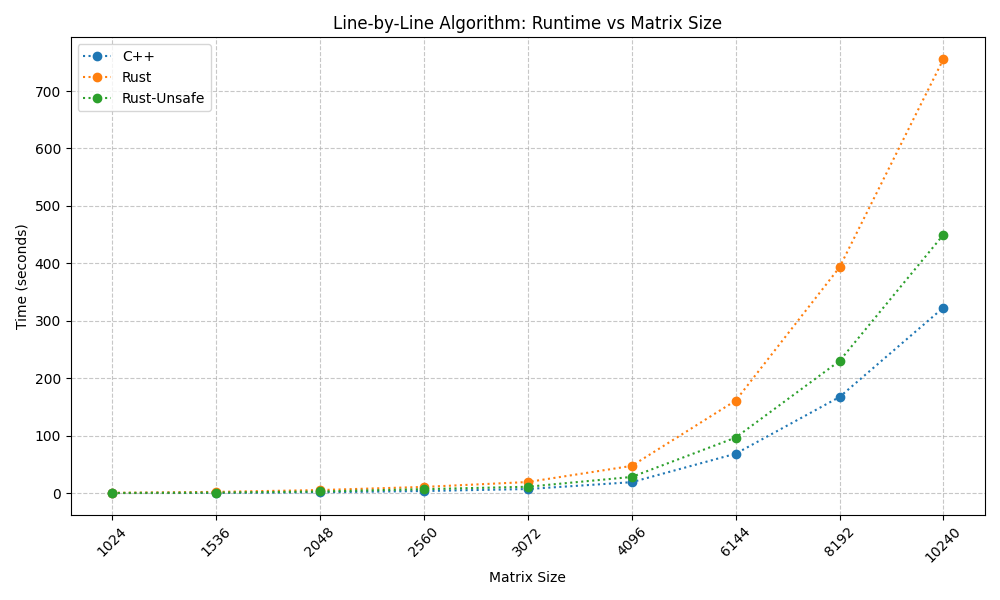
\includegraphics[width=0.85\linewidth]{../results/pythonGraphs/graphImgs/time_line.png}
  \caption{Execution time (s) of the \textit{LLA} for C++ and Rust variants.}
  \label{fig:time_line}
\end{figure}

The most immediate observation is the dramatic improvement over the
\textit{BMMA} (Table~\ref{tab:time_line}, Figure~\ref{fig:time_line}): simply reordering the loop traversal from \texttt{ijk} to
\texttt{ikj} yields a $\sim$17.5$\times$ speedup for C++ at $n = 1024$
(from 0.95 to 16.6\,GFlop/s). This improvement stems entirely from improved
spatial locality --- the reordered loop accesses the second matrix
row-by-row rather than column-by-column, dramatically reducing cache misses.

The language gap is now substantial and clearly visible in Figure~\ref{fig:time_line}. C++
reaches 16.6\,GFlop/s at $n = 1024$, Rust unsafe 6.5\,GFlop/s, and Rust
safe only 3.4\,GFlop/s (Table~\ref{tab:time_line}). This hierarchy is explained by vectorisation: GCC
with \texttt{-O3 -march=native} auto-vectorises the innermost $j$-loop using
AVX2 SIMD instructions, while Rust safe's bounds checks prevent the compiler
from doing the same. Rust unsafe's \texttt{get\_unchecked} removes those
checks and enables partial vectorisation, roughly doubling throughput over
safe Rust, though GCC still generates superior code overall.

Beyond $n = 1536$, throughput declines steadily for all implementations as
the working set exceeds L1 cache capacity, before stabilising at
6.5--7.2\,GFlop/s for C++ at $n \geq 4096$, where L3 prefetching sustains
adequate memory bandwidth. Rust safe plateaus around 2.8--3.4\,GFlop/s and
Rust unsafe around 4.8--5.2\,GFlop/s across the same range, maintaining
consistent relative gaps throughout.

\begin{table}[H]
  \centering
  \caption{Absolute L1 and L2 cache misses (\texttt{perf}) -- \textit{LLA},
           representative sizes.}
  \label{tab:perf_line}
  \begin{tabular}{llrr}
    \toprule
    \textbf{Implementation} & \textbf{Size} & \textbf{L1 misses} & \textbf{L2 misses} \\
    \midrule
    C++         & 1024 &  68{,}347{,}062     &  13{,}594{,}759   \\
    C++         & 3072 &  2{,}383{,}808{,}702 & 951{,}744{,}599   \\
    Rust safe   & 1024 &   1{,}916{,}497     &     246{,}122     \\
    Rust safe   & 3072 & 213{,}260{,}229     &   9{,}134{,}707   \\
    Rust unsafe & 1024 &  64{,}168{,}534     &   7{,}404{,}176   \\
    Rust unsafe & 3072 & 246{,}816{,}936     &  37{,}530{,}874   \\
    \bottomrule
  \end{tabular}
\end{table}

\begin{figure}[H]
  \centering
  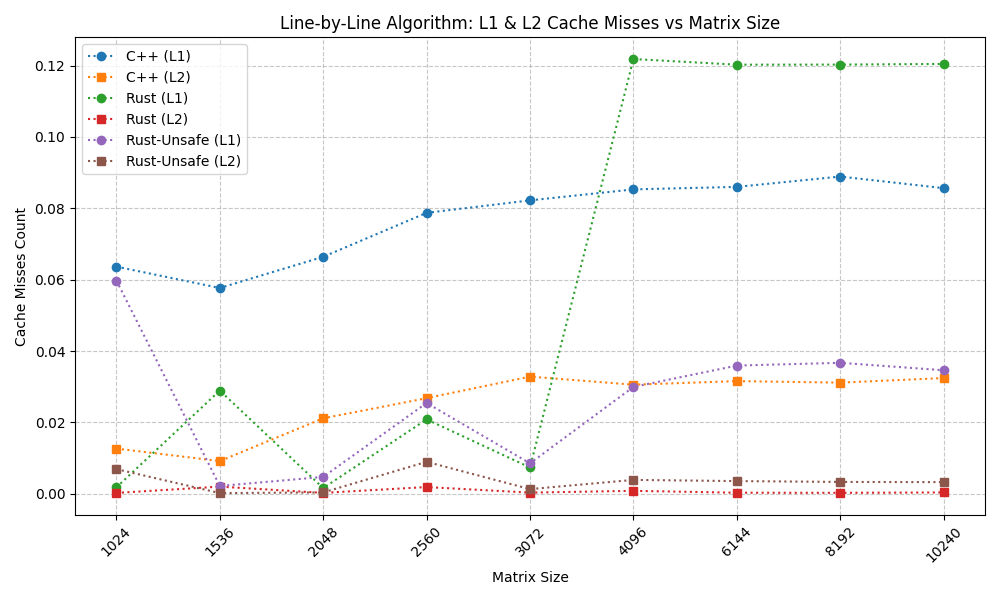
\includegraphics[width=0.85\linewidth]{../results/pythonGraphs/graphImgs/misses_line.png}
  \caption{Normalised L1 and L2 cache misses of the \textit{LLA} -- C++ and
           Rust variants.}
  \label{fig:misses_line}
\end{figure}

Compared to the \textit{BMMA}, where normalised miss rates (Equation~\ref{eq:norm_misses}) sat between 0.83
and 1.00 (Figure~\ref{fig:misses_basic}), the \textit{LLA} brings them down to a range of 0.00 to 0.12
(Figure~\ref{fig:misses_line}) ---
a dramatic reduction that directly explains the order-of-magnitude improvement
in throughput. The algorithm is no longer nearly fully memory-bound; the
reordered access pattern allows the hardware prefetcher to sustain most
accesses from cache.

C++ consistently exhibits the highest normalised L1 miss rate
($\sim$0.06--0.09), which may seem counterintuitive given its superior
performance. This apparent paradox arises from AVX2 vectorisation: wide SIMD
loads operate on multiple elements simultaneously, generating more counted L1
cache events per instruction than scalar loads do, even though the effective
memory bandwidth consumed is similar or better. In other words, more L1 events
are recorded precisely because C++ is doing more useful work per cycle.

Rust safe, despite being the slowest implementation, reports the lowest
normalised miss rates (near zero for L2 throughout). Its scalar inner loop
issues one load per element with a regular stride, which the hardware
prefetcher handles efficiently without those accesses being recorded as demand
misses. This confirms that Rust safe's low miss count reflects its scalar
access granularity rather than superior cache utilisation.

Rust unsafe sits between the two, with L1 miss rates around 0.00--0.04 and
slightly higher L2 miss rates, consistent with its partial vectorisation and
intermediate throughput.

L2 miss rates are low across all implementations (at most $\sim$0.035 for
C++), confirming that L2 successfully absorbs the majority of L1 misses and
that main memory pressure is modest --- a stark contrast to the \textit{BMMA}.

% ─────────────────────────────────────────────────────────────────────────────
\subsection{Block-Oriented Algorithm -- \textit{BOA}}
\label{subsec:res_block}
% ─────────────────────────────────────────────────────────────────────────────

\begin{table}[H]
  \centering
  \caption{Execution time (s) and GFlop/s -- \textit{BOA}, C++.}
  \label{tab:time_block_cpp}
  \sisetup{round-mode=places, round-precision=3}
  \begin{tabular}{
      S[table-format=5.0, round-precision=0]
      S[table-format=6.3] S[table-format=5.3]
      S[table-format=6.3] S[table-format=5.3]
      S[table-format=6.3] S[table-format=5.3]
    }
    \toprule
    & \multicolumn{2}{c}{\textbf{Block 128}} & \multicolumn{2}{c}{\textbf{Block 256}} & \multicolumn{2}{c}{\textbf{Block 512}} \\
    \cmidrule(lr){2-3}\cmidrule(lr){4-5}\cmidrule(lr){6-7}
    {Size ($n$)} & {Time (s)} & {GFlop/s} & {Time (s)} & {GFlop/s} & {Time (s)} & {GFlop/s} \\
    \midrule
    4096  &  10.407 & 13.206 &   9.839 & 13.972 &   9.217 & 14.919 \\
    6144  &  26.938 & 17.229 &  33.057 & 14.028 &  29.701 & 15.611 \\
    8192  &  91.191 & 12.040 &  84.134 & 13.041 & 113.682 &  9.650 \\
    10240 & 124.644 & 17.230 & 153.296 & 14.005 & 140.389 & 15.293 \\
    \bottomrule
  \end{tabular}
\end{table}

\begin{table}[H]
  \centering
  \caption{Execution time (s) and GFlop/s -- \textit{BOA}, Rust safe.}
  \label{tab:time_block_rust_safe}
  \sisetup{round-mode=places, round-precision=3}
  \begin{tabular}{
      S[table-format=5.0, round-precision=0]
      S[table-format=6.3] S[table-format=5.3]
      S[table-format=6.3] S[table-format=5.3]
      S[table-format=6.3] S[table-format=5.3]
    }
    \toprule
    & \multicolumn{2}{c}{\textbf{Block 128}} & \multicolumn{2}{c}{\textbf{Block 256}} & \multicolumn{2}{c}{\textbf{Block 512}} \\
    \cmidrule(lr){2-3}\cmidrule(lr){4-5}\cmidrule(lr){6-7}
    {Size ($n$)} & {Time (s)} & {GFlop/s} & {Time (s)} & {GFlop/s} & {Time (s)} & {GFlop/s} \\
    \midrule
    4096  &  43.525 &  3.158 &  44.908 &  3.060 &  43.962 &  3.125 \\
    6144  & 142.106 &  3.267 & 151.853 &  3.056 & 147.249 &  3.153 \\
    8192  & 361.912 &  3.036 & 370.392 &  2.966 & 417.558 &  2.630 \\
    10240 & 668.264 &  3.215 & 704.150 &  3.053 & 683.027 &  3.145 \\
    \bottomrule
  \end{tabular}
\end{table}

\begin{table}[H]
  \centering
  \caption{Execution time (s) and GFlop/s -- \textit{BOA}, Rust unsafe.}
  \label{tab:time_block_rust_unsafe}
  \sisetup{round-mode=places, round-precision=3}
  \begin{tabular}{
      S[table-format=5.0, round-precision=0]
      S[table-format=6.3] S[table-format=5.3]
      S[table-format=6.3] S[table-format=5.3]
      S[table-format=6.3] S[table-format=5.3]
    }
    \toprule
    & \multicolumn{2}{c}{\textbf{Block 128}} & \multicolumn{2}{c}{\textbf{Block 256}} & \multicolumn{2}{c}{\textbf{Block 512}} \\
    \cmidrule(lr){2-3}\cmidrule(lr){4-5}\cmidrule(lr){6-7}
    {Size ($n$)} & {Time (s)} & {GFlop/s} & {Time (s)} & {GFlop/s} & {Time (s)} & {GFlop/s} \\
    \midrule
    4096  &  23.482 &  5.863 &  22.177 &  6.208 &  22.302 &  6.173 \\
    6144  &  69.761 &  6.652 &  74.771 &  6.208 &  73.463 &  6.318 \\
    8192  & 190.044 &  5.780 & 186.167 &  5.900 & 248.884 &  4.413 \\
    10240 & 329.042 &  6.527 & 347.999 &  6.173 & 340.043 &  6.317 \\
    \bottomrule
  \end{tabular}
\end{table}

\begin{figure}[H]
  \centering
  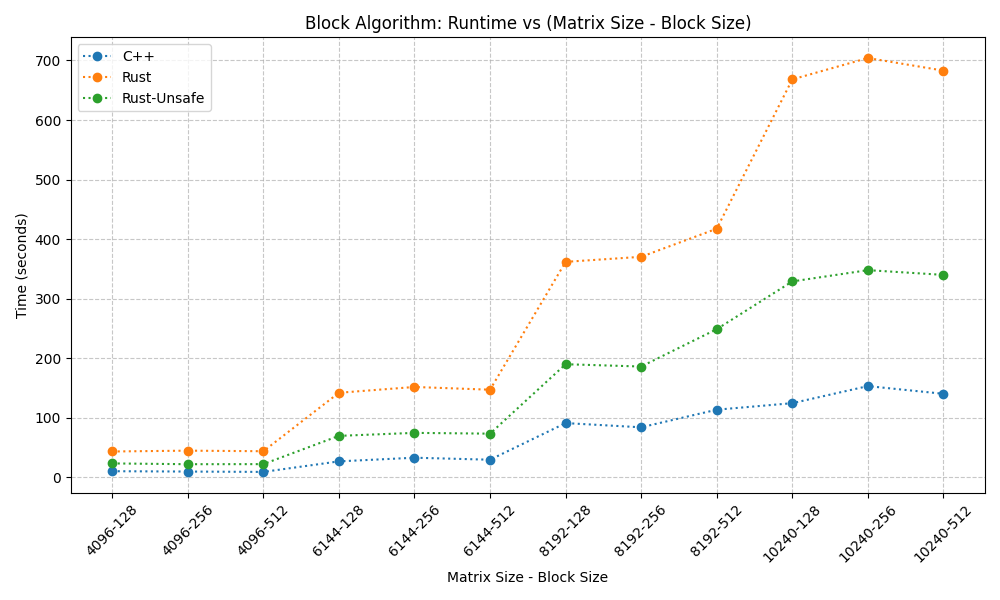
\includegraphics[width=0.85\linewidth]{../results/pythonGraphs/graphImgs/time_block.png}
  \caption{Execution time (s) of the \textit{BOA} for C++ and Rust variants
           across block sizes 128, 256, and 512.}
  \label{fig:time_block}
\end{figure}

Block tiling delivers a further $\sim$2$\times$ improvement over the
\textit{LLA} for C++ at large matrix sizes (Tables~\ref{tab:time_block_cpp}--\ref{tab:time_block_rust_unsafe},
Figure~\ref{fig:time_block}), reaching 13--17\,GFlop/s versus
6.6--7.2\,GFlop/s. By dividing the matrices into sub-blocks that fit within
L2 cache, the algorithm maximises data reuse and reduces the number of times
each element needs to be fetched from slower memory levels.

For most cases, block sizes 128 and 256 consistently outperform block 512 across most
sizes (Tables~\ref{tab:time_block_cpp}--\ref{tab:time_block_rust_unsafe}). This is explained by the block's working
set size: three blocks of side $b$ require $3b^2$ doubles, occupying
$3 \times 512^2 \times 8 = 6.0$\,MB, which spills into L3 cache. Blocks 128
and 256 fit comfortably within the 2\,MB L2 cache and therefore sustain higher
throughput.

Rust unsafe improves over safe Rust ($\sim$6.0--6.7\,GFlop/s), 
reflecting partial vectorisation, but remains well
below C++ throughout.

\begin{table}[H]
  \centering
  \caption{Absolute L1 and L2 cache misses (\texttt{perf}) -- \textit{BOA},
           C++, $n = 8192$.}
  \label{tab:perf_block}
  \begin{tabular}{lrr}
    \toprule
    \textbf{Block size} & \textbf{L1 misses} & \textbf{L2 misses} \\
    \midrule
    128 & 39{,}666{,}483{,}471 & 31{,}186{,}589{,}244 \\
    256 & 35{,}560{,}127{,}785 & 17{,}511{,}891{,}888 \\
    512 & 34{,}838{,}609{,}458 & 11{,}609{,}694{,}378 \\
    \bottomrule
  \end{tabular}
\end{table}

\begin{figure}[H]
  \centering
  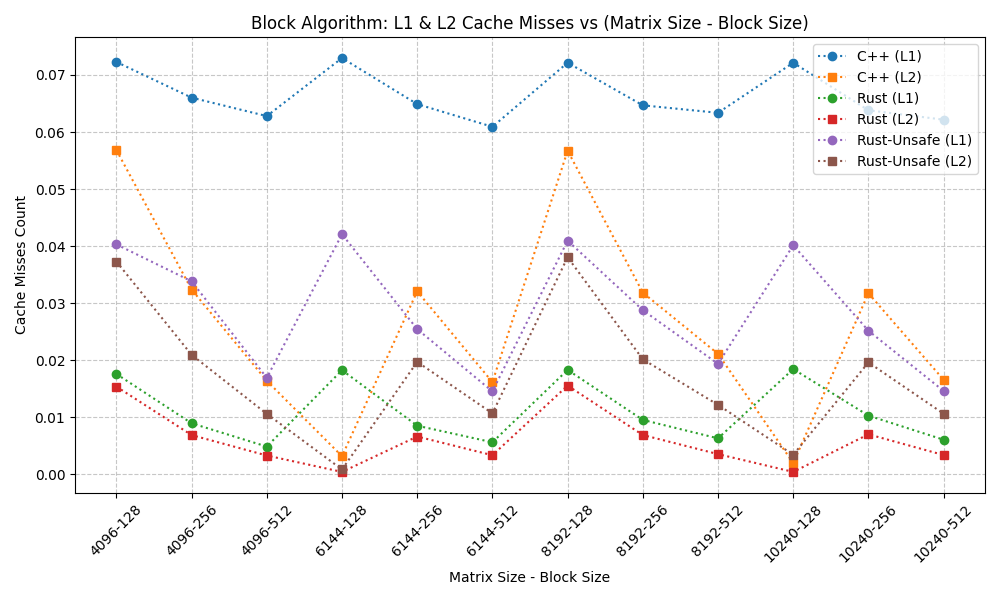
\includegraphics[width=0.85\linewidth]{../results/pythonGraphs/graphImgs/misses_block.png}
  \caption{Normalised L1 and L2 cache misses of the \textit{BOA} -- C++ and
           Rust variants, across block sizes.}
  \label{fig:misses_block}
\end{figure}

The normalised miss rates for the \textit{BOA} sit in the range of 0.00 to
0.07 (Figure~\ref{fig:misses_block}, Table~\ref{tab:perf_block}), substantially lower than the \textit{BMMA} (0.83--1.00,
Figure~\ref{fig:misses_basic}) and modestly lower than the \textit{LLA} (0.00--0.12,
Figure~\ref{fig:misses_line}). This confirms that block tiling
further reduces cache pressure by improving data reuse within each block, even
if the gains are more incremental than the step from \textit{BMMA} to
\textit{LLA}.

C++ consistently exhibits the highest normalised L1 miss rates
($\sim$0.06--0.07), for the same reason observed in the \textit{LLA}: AVX2
SIMD loads generate more counted L1 cache events per unit of work than scalar
loads, reflecting higher data throughput rather than poorer cache behaviour.

A clear trend is visible across block sizes (Table~\ref{tab:perf_block}, Figure~\ref{fig:misses_block}): larger blocks reduce L2 miss
rates significantly (block 512 at $n = 8192$ shows roughly one third the L2
misses of block 128), because larger blocks amortise the cost of bringing data
into cache over more reuse operations. However, this benefit is offset when the
block exceeds L2 capacity, as seen with block 512, where the working set spills
into L3 and L1 miss rates remain comparably high to the smaller blocks.

Rust safe reports near-zero L2 miss rates across all configurations,
consistent with its scalar access pattern and the hardware prefetcher's ability
to absorb demand misses. Rust unsafe sits between the two, with L1 miss rates
around 0.01--0.04 and low but non-negligible L2 miss rates, tracking its
partial vectorisation behaviour.

The oscillating pattern visible in the graph across the $x$-axis groupings
(particularly for Rust unsafe L1 and C++ L2) reflects the interaction between
block size and matrix size: each group of three points represents the same $n$
with blocks 128, 256, 512 respectively, and the within-group variation captures
how sensitive each implementation is to the choice of block size.

% ─────────────────────────────────────────────────────────────────────────────
\subsection{BMMA and LLA - Overlap}
\label{sec:overlap}
% ─────────────────────────────────────────────────────────────────────────────

Taking into consideration the fact that BMMA and LLA shared testing sizes, graphs displaying the execution time and cache misses
for both we generated. These allow to better display the proportions of the improvements the later provides.

\begin{figure}[H]
  \centering
  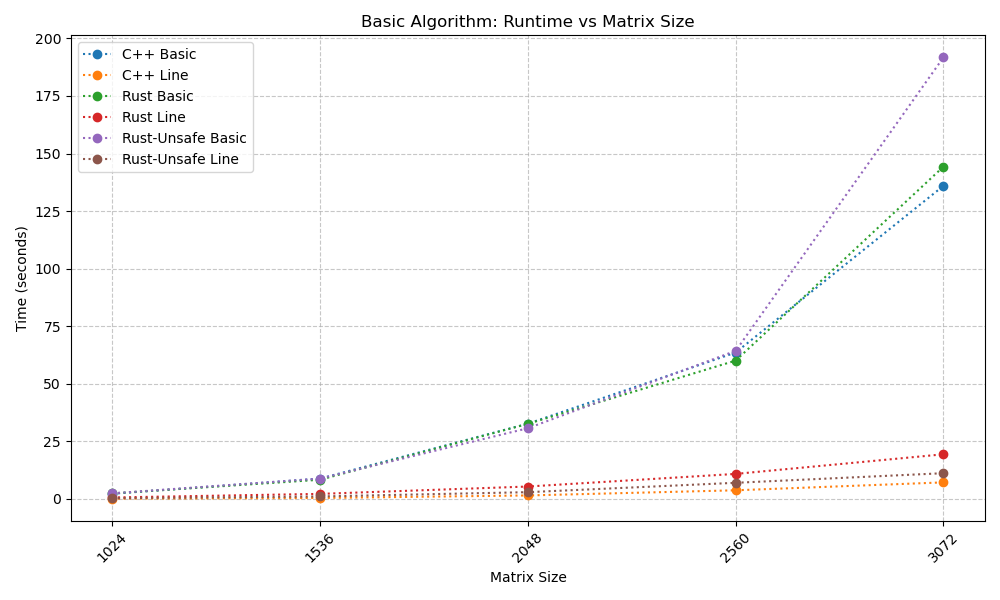
\includegraphics[width=0.85\linewidth]{../graphImgs/time_overlap.png}
  \caption{Execution time (s) of the \textit{BMMA} and \textit{LLA} for C++ and Rust variants
           across matrix sizes 1024, 1536, 2048, 2560 and 3072.}
  \label{fig:time_overlap}
\end{figure}

\begin{figure}[H]
  \centering
  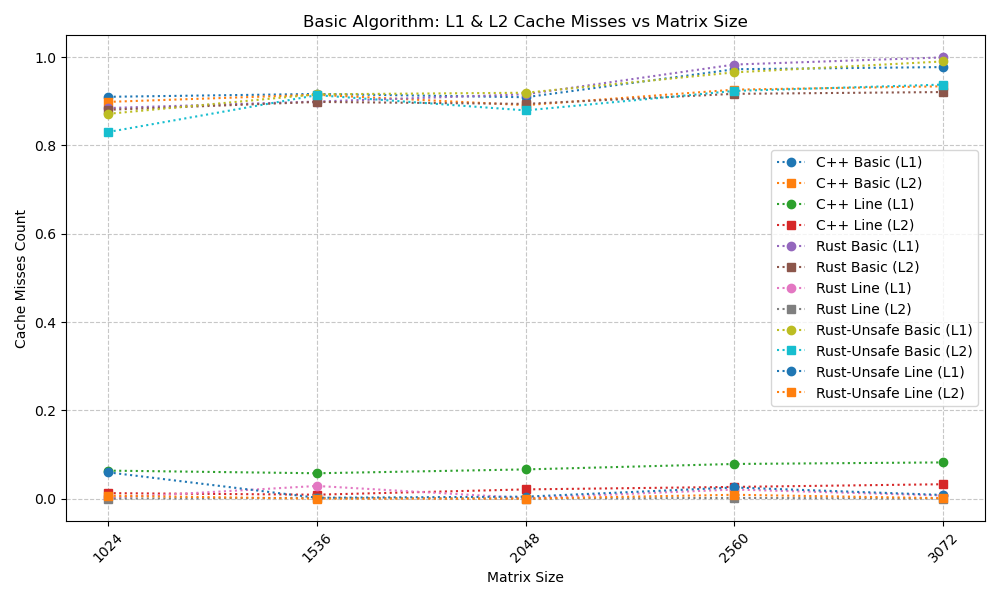
\includegraphics[width=0.85\linewidth]{../graphImgs/misses_overlap.png}
  \caption{Normalised L1 and L2 cache misses of the \textit{BMMA} and \textit{LLA} for C++ and Rust variants
           across matrix sizes 1024, 1536, 2048, 2560 and 3072.}
  \label{fig:misses_overlap}
\end{figure}

As shown in Figure~\ref{fig:time_overlap}, the execution time of the \textit{BMMA} grows exponentially and dominates the graph,
 whereas the \textit{LLA} execution times appear nearly flat by comparison. This visual scaling dramatically emphasizes the 
 $\sim$17.5$\times$ speedup discussed in Section~\ref{subsec:res_line}. While the \textit{BMMA} struggles under the weight of memory 
 latency, reaching nearly 200 seconds for the unsafe Rust variant at $n=3072$, the \textit{LLA} completes the same workload in a fraction 
 of the time across all languages.

Figure~\ref{fig:misses_overlap} provides the direct mechanical explanation for this runtime disparity. The normalized cache miss rates are 
completely bifurcated: the \textit{BMMA} implementations cluster at the top of the chart with miss rates between 0.83 and 1.00, meaning 
almost every memory access results in a cache miss. Conversely, the \textit{LLA} implementations cluster tightly at the bottom, with miss 
rates hovering near zero. This stark contrast definitively proves that the massive performance gap is entirely attributable to the improved 
spatial locality achieved by simply reordering the loop traversal.

% ─────────────────────────────────────────────────────────────────────────────
\section{Multi-Core Results and Discussion}
\label{sec:multicore_results}
% ─────────────────────────────────────────────────────────────────────────────

% ─────────────────────────────────────────────────────────────────────────────
\subsection{Parallelisation Strategies}
\label{subsec:par_strategies}
% ─────────────────────────────────────────────────────────────────────────────

Three parallelisation strategies were designed and evaluated, each applying
OpenMP directives differently to the loop structure of the matrix multiplication
algorithms studied in Part 1.

\paragraph{Parallel Outer Loop.}
The outermost $i$-loop of the \texttt{ijk} algorithm is distributed across
threads via \texttt{\#pragma omp parallel for}. Each thread computes
contiguous rows of $C$, so writes and $A$-reads are private to each thread.
However, all threads still read every column of $B$ with poor column-stride
access, so L3 bandwidth becomes the bottleneck regardless of thread count.

\begin{lstlisting}[style=cppstyle, caption={Parallel outer loop (\texttt{ijk})}]
#pragma omp parallel for
for (int i = 0; i < n; i++)
    for (int j = 0; j < n; j++) {
        double temp = 0;
        for (int k = 0; k < n; k++)
            temp += A[i*n+k] * B[k*n+j];
        C[i*n+j] = temp;
    }
\end{lstlisting}

\paragraph{Parallel Inner Loop.}
A parallel region wraps all three loops; only the innermost $k$-loop is
workshared. Each thread computes a partial sum, but then all threads write
their partial result to the same \texttt{C[i*n+j]} entry, creating a race
condition. This is \textbf{incorrect} and produces wrong results. Performance
is also poor, as the $n^2$ iterations of the outer loops each introduce an
implicit synchronisation barrier at the end of the workshared $k$-loop.

\begin{lstlisting}[style=cppstyle, caption={Parallel inner loop}]
#pragma omp parallel
for (int i = 0; i < n; i++)
    for (int j = 0; j < n; j++) {
        double temp = 0;
        #pragma omp for
        for (int k = 0; k < n; k++)
            temp += A[i*n+k] * B[k*n+j];
        C[i*n+j] = temp;
    }
\end{lstlisting}

\paragraph{Parallel Line.}
\texttt{\#pragma omp parallel for} is applied to the $i$-loop of the
cache-friendly \texttt{ikj} algorithm. Each thread owns non-overlapping rows
of $C$ and $A$, reads $B$ with row-major locality, and writes without
conflicts. This is both correct and cache-efficient, and serves as the
foundation for the scalability analysis that follows.

\begin{lstlisting}[style=cppstyle, caption={Parallel Line}]
#pragma omp parallel for
for (int i=0; i<n; i++)
    for (int k=0; k<n; k++)
        for (int j=0; j<n; j++)
            C(i,j)+=A(i,k)*B(k,j)
\end{lstlisting}

% ─────────────────────────────────────────────────────────────────────────────
\subsection{Parallel Outer Loop vs. Parallel Inner Loop vs. Parallel Line
            (4 Threads, n from 1024 to 3072)}
\label{subsec:par_comparison}
% ─────────────────────────────────────────────────────────────────────────────

\begin{table}[H]
  \centering
  \caption{Execution time (s) and GFlop/s -- parallelisation strategies,
           4 threads.}
  \label{tab:step1}
  \sisetup{round-mode=places, round-precision=3}
  \begin{tabular}{
      S[table-format=4.0, round-precision=0]
      S[table-format=6.3] S[table-format=5.3]
      S[table-format=6.3] S[table-format=5.3]
      S[table-format=5.3] S[table-format=5.3]
    }
    \toprule
    & \multicolumn{2}{c}{\textbf{Par Outer Loop}} &
      \multicolumn{2}{c}{\textbf{Par Inner Loop}} &
      \multicolumn{2}{c}{\textbf{Par Line}} \\
    \cmidrule(lr){2-3}\cmidrule(lr){4-5}\cmidrule(lr){6-7}
    {$n$} & {Time (s)} & {GFlop/s} & {Time (s)} & {GFlop/s} &
            {Time (s)} & {GFlop/s} \\
    \midrule
    1024 &  0.575 &  3.735 &  2.219 & 0.968 & 0.114 & 18.833 \\
    1536 &  1.991 &  3.641 &  5.400 & 1.342 & 0.370 & 19.587 \\
    2048 &  5.031 &  3.415 & 18.796 & 0.914 & 1.475 & 11.647 \\
    2560 & 18.542 &  1.810 & 29.759 & 1.128 & 2.858 & 11.740 \\
    3072 & 33.445 &  1.734 & 70.927 & 0.817 & 4.909 & 11.814 \\
    \bottomrule
  \end{tabular}
\end{table}

\begin{figure}[H]
  \centering
  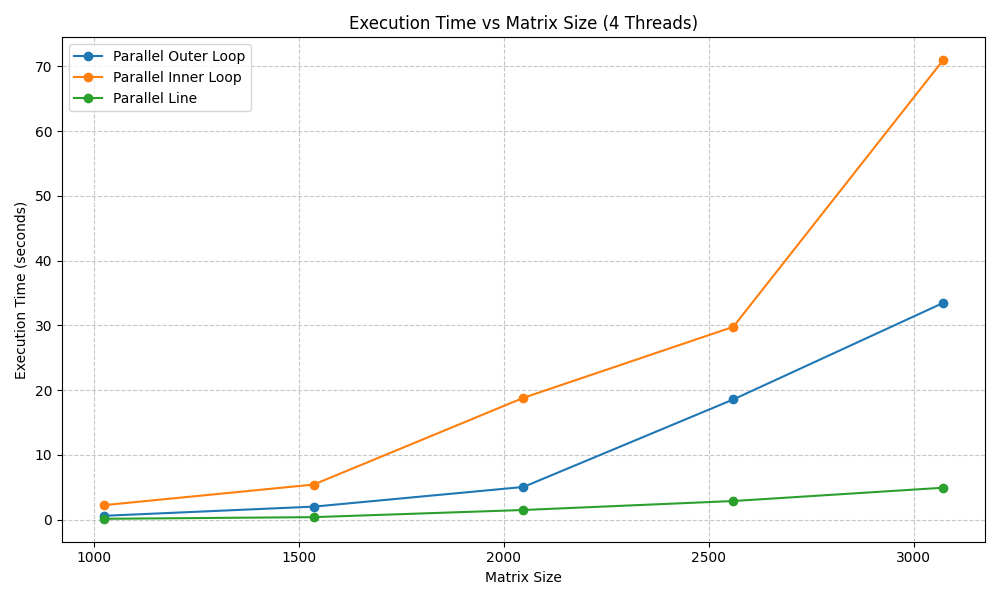
\includegraphics[width=0.85\linewidth]{../results/pythonGraphs/graphImgs/time_step1.png}
  \caption{Execution time (s) of parallelisation strategies (4 threads) vs.\
           matrix size.}
  \label{fig:time_step1}
\end{figure}

\begin{figure}[H]
  \centering
  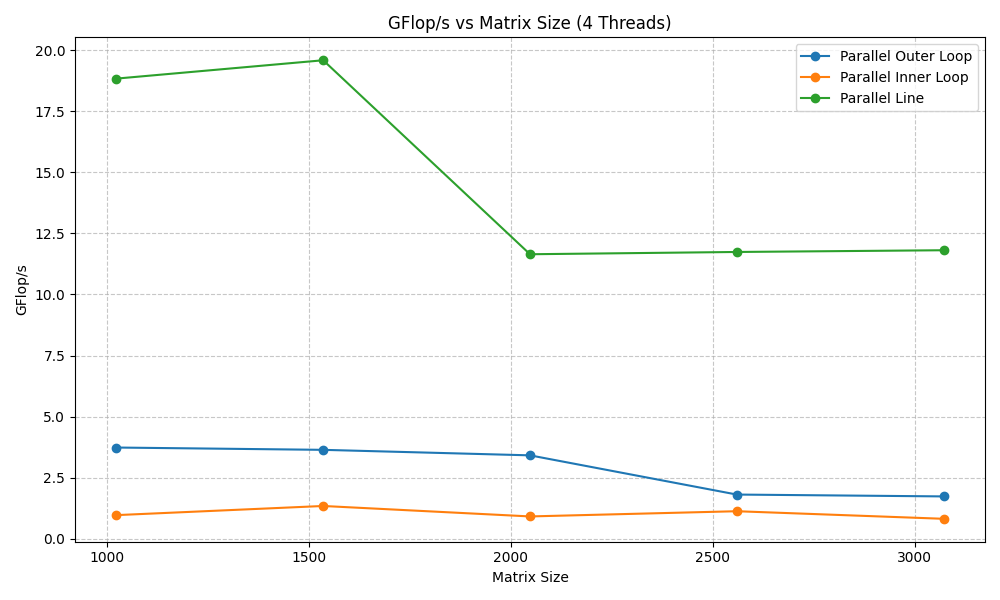
\includegraphics[width=0.85\linewidth]{../results/pythonGraphs/graphImgs/gflops_step1.png}
  \caption{GFlop/s of parallelisation strategies (4 threads) vs.\ matrix
           size.}
  \label{fig:gflops_step1}
\end{figure}

The results confirm the theoretical expectations laid out in the previous
section (Table~\ref{tab:step1}, Figures~\ref{fig:time_step1}~and~\ref{fig:gflops_step1}).
Parallel Line is the clear winner, achieving 11.8--19.6\,GFlop/s at
4 threads --- a $\sim$$1.1$--$1.5\times$ improvement over single-core
\textit{LLA} at the same sizes, and an order of magnitude above the other two
strategies.

Parallel Outer Loop reaches only 1.7--3.7\,GFlop/s, which is an improvement
over the single-core \textit{BMMA} (0.4--0.95\,GFlop/s) but remains far below
single-core \textit{LLA} (6.6--16.6\,GFlop/s). Distributing the $i$-loop
across threads reduces per-thread work, but the column-stride access pattern
on $B$ is unchanged --- each thread still generates the same cache-unfriendly
memory accesses, and the threads now compete for shared L3 bandwidth,
compounding the bottleneck.

Parallel Inner Loop is both incorrect and the slowest of the three, achieving
only 0.8--1.3\,GFlop/s. The race condition on \texttt{C[i*n+j]} produces
wrong results, and the $n^2$ implicit synchronisation barriers introduced by
the inner workshared loop create enormous overhead that grows rapidly with
matrix size, as clearly visible in Figure~\ref{fig:time_step1}.

Parallel Line avoids both problems by distributing independent row-chunks
across threads on an already cache-friendly access pattern. The drop from
$\sim$19\,GFlop/s at $n \leq 1536$ to $\sim$11.8\,GFlop/s at $n \geq 2048$
mirrors the same cache pressure transition observed in the single-core
\textit{LLA}, now shifted slightly by the combined per-thread working sets
exceeding L2 capacity.

% ─────────────────────────────────────────────────────────────────────────────
\subsection{Parallel Line Scalability (n = 8192, 4 to 24 Threads)}
\label{subsec:par_scalability}
% ─────────────────────────────────────────────────────────────────────────────

Having established Parallel Line as the most effective strategy, the analysis
was extended to evaluate scalability at $n = 8192$ across thread counts from 4
to 24, and to compare three variants of the directive applied to the innermost
$j$-loop:

\begin{itemize}
  \item \textbf{Parallel Line} --- baseline, \texttt{\#pragma omp parallel for}
        on the $i$-loop only.
  \item \textbf{Parallel + SIMD} --- adds \texttt{\#pragma omp simd} to the
        innermost $j$-loop, hinting the compiler to apply AVX2 vectorisation
        in addition to thread parallelism.
  \item \textbf{Parallel + Collapse(2)} --- uses \texttt{collapse(2)} to merge
        the $i$ and $k$ loops into a single $n^2$-iteration space, exposing
        more parallelism at the cost of breaking per-thread row-reuse of $B$.
\end{itemize}

\begin{table}[H]
  \centering
  \caption{Execution time (s) -- Parallel Line variants at $n = 8192$.}
  \label{tab:step2_time}
  \sisetup{round-mode=places, round-precision=3}
  \begin{tabular}{
      S[table-format=2.0, round-precision=0]
      S[table-format=6.3]
      S[table-format=6.3]
      S[table-format=6.3]
    }
    \toprule
    {Threads} & {Par Line (s)} & {Par + SIMD (s)} & {Par + Collapse(2) (s)} \\
    \midrule
     4 & 100.591 &  88.960 &  99.781 \\
     8 &  76.342 &  63.635 &  75.137 \\
    12 &  63.136 &  53.378 &  57.462 \\
    16 &  55.638 &  55.058 &  57.981 \\
    20 &  57.971 &  50.464 &  57.360 \\
    24 &  55.819 &  47.134 &  54.728 \\
    \bottomrule
  \end{tabular}
\end{table}

\begin{table}[H]
  \centering
  \caption{GFlop/s and Speedup -- Parallel Line variants at $n = 8192$
           (baseline: Par Line, 4 threads, 100.591\,s).}
  \label{tab:step2_gflops}
  \begin{tabular}{
      S[table-format=2.0, round-precision=0]
      S[table-format=5.3] S[table-format=4.3]
      S[table-format=5.3] S[table-format=4.3]
      S[table-format=5.3] S[table-format=4.3]
    }
    \toprule
    & \multicolumn{2}{c}{\textbf{Par Line}} &
      \multicolumn{2}{c}{\textbf{Par + SIMD}} &
      \multicolumn{2}{c}{\textbf{Par + Collapse(2)}} \\
    \cmidrule(lr){2-3}\cmidrule(lr){4-5}\cmidrule(lr){6-7}
    {Threads} & {GFlop/s} & {Speedup} & {GFlop/s} & {Speedup} &
               {GFlop/s} & {Speedup} \\
    \midrule
     4 & 10.930 & 1.000 & 12.360 & 1.131 & 11.019 & 1.008 \\
     8 & 14.402 & 1.317 & 17.279 & 1.581 & 14.632 & 1.339 \\
    12 & 17.415 & 1.593 & 20.600 & 1.885 & 19.133 & 1.750 \\
    16 & 19.765 & 1.808 & 19.971 & 1.826 & 18.963 & 1.735 \\
    20 & 18.967 & 1.735 & 21.790 & 1.993 & 19.170 & 1.754 \\
    24 & 19.699 & 1.802 & 23.326 & 2.134 & 20.091 & 1.838 \\
    \bottomrule
  \end{tabular}
\end{table}

\begin{figure}[H]
  \centering
  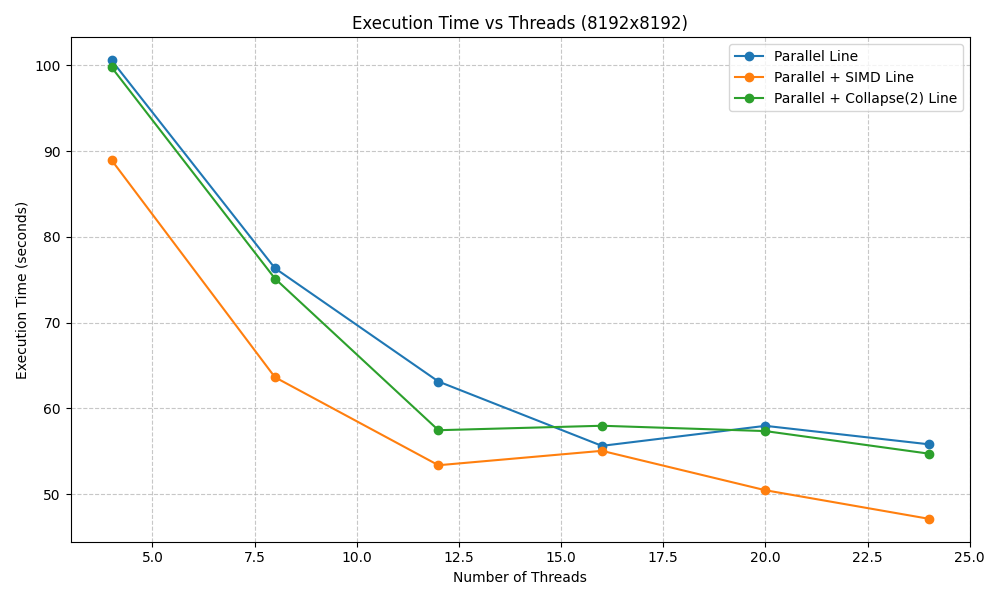
\includegraphics[width=0.85\linewidth]{../results/pythonGraphs/graphImgs/time_step2.png}
  \caption{Execution time (s) of Parallel Line variants vs.\ thread count at
           $n = 8192$.}
  \label{fig:time_step2}
\end{figure}

\begin{figure}[H]
  \centering
  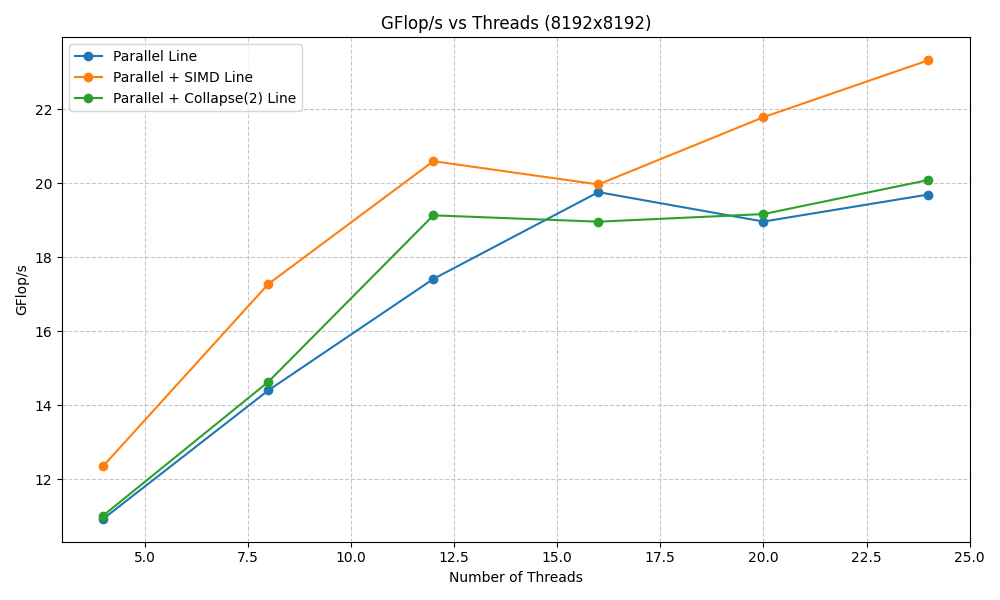
\includegraphics[width=0.85\linewidth]{../results/pythonGraphs/graphImgs/gflops_step2.png}
  \caption{GFlop/s of Parallel Line variants vs.\ thread count at $n = 8192$.}
  \label{fig:gflops_step2}
\end{figure}

\begin{figure}[H]
  \centering
  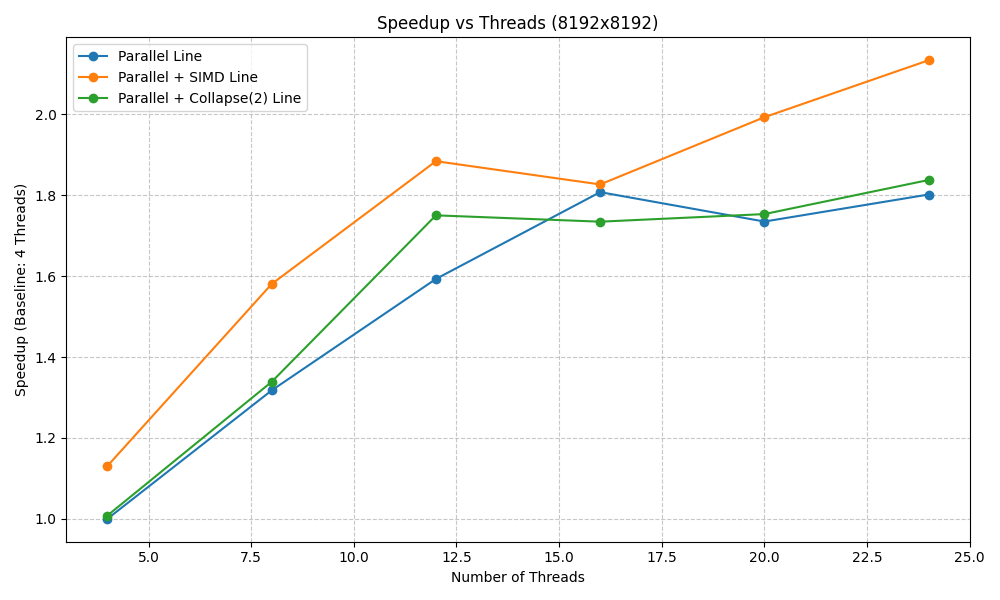
\includegraphics[width=0.85\linewidth]{../results/pythonGraphs/graphImgs/speedup_step2.png}
  \caption{Speedup of Parallel Line variants vs.\ thread count at $n = 8192$
           (baseline: Par Line, 4 threads).}
  \label{fig:speedup_step2}
\end{figure}

All three variants reduce execution time as thread count increases from 4 to
24, but none approach linear scaling, and all plateau well before 24 threads
(Tables~\ref{tab:step2_time}~and~\ref{tab:step2_gflops}).
This is visible in both Figures~\ref{fig:time_step2}~and~\ref{fig:speedup_step2}, where the curves
flatten significantly beyond 12--16 threads.

Parallel Line scales from 10.9\,GFlop/s at 4 threads to 19.7\,GFlop/s at 24
threads, a $1.80\times$ speedup (Table~\ref{tab:step2_gflops}). The gains are consistent up to 12 threads,
after which performance stagnates and even dips at 20 threads before
recovering slightly at 24. This non-monotonic behaviour is characteristic of
heterogeneous CPU topology: once threads spill from performance cores onto
efficiency cores, per-thread throughput drops, and the scheduler overhead
partially offsets the added parallelism.

Parallel + SIMD is the strongest performer at every thread count (Table~\ref{tab:step2_gflops},
Figure~\ref{fig:gflops_step2}), reaching
23.3\,GFlop/s at 24 threads ($2.13\times$ speedup over the 4-thread baseline).
The SIMD hint enables AVX2 vectorisation on the innermost $j$-loop, adding a
consistent $\sim$15--18\% throughput advantage over plain Parallel Line across
all thread counts. Crucially, the SIMD benefit compounds with thread scaling:
the gap between Parallel + SIMD and the others widens as thread count
increases, suggesting that vectorisation and parallelism are largely
orthogonal and additive at this problem size.

Parallel + Collapse(2) performs nearly identically to plain Parallel Line
throughout (Table~\ref{tab:step2_gflops}), with $\sim$20.1\,GFlop/s at 24 threads ($1.84\times$ speedup), despite
flattening the $i$ and $k$ loops into $n^2 \approx 67$\,million iterations.
The theoretical benefit of exposing more parallelism is negated by the fact
that collapsing the loops breaks the per-thread row-reuse of $B$: threads no
longer operate on contiguous rows, destroying the spatial locality that makes
Parallel Line efficient. Load balance improves, but cache behaviour degrades
by roughly the same amount.

The overall speedup ceiling of $\sim$$2\times$ relative to single-core
\textit{LLA} (167.4\,s at $n = 8192$) is modest (Table~\ref{tab:step2_gflops},
Figure~\ref{fig:speedup_step2}). Parallel + SIMD at 24
threads (47.1\,s) yields a $3.55\times$ speedup over single-core, but at an
efficiency of only $\sim$15\%. The primary bottlenecks are memory bandwidth
--- the $n = 8192$ working set is $\sim$1.5\,GB, far exceeding all cache
levels --- and the heterogeneous P/E-core topology of the test CPU, which
limits the effective thread count before diminishing returns set in.

% ─────────────────────────────────────────────────────────────────────────────
\section{Conclusion}
\label{sec:conclusion}
% ─────────────────────────────────────────────────────────────────────────────

This report set out to investigate how the memory hierarchy affects processor
performance during matrix multiplication, and to evaluate how algorithmic
design, language choice, and parallelisation strategy each contribute to
computational throughput. The results, taken together, paint a consistent and
instructive picture.

The single most impactful optimisation across the entire study was loop
reordering. Simply changing the traversal order from \texttt{ijk} to
\texttt{ikj} --- at zero additional computational cost --- yielded a
$\sim$$17.5\times$ speedup for C++ at $n = 1024$ (Table~\ref{tab:time_line}),
reducing normalised L1 miss rates from $\sim$0.95 to $\sim$0.06
(Figures~\ref{fig:misses_basic}~and~\ref{fig:misses_line}). This result alone illustrates the
central thesis of the report: algorithmic memory access patterns, not raw
computational complexity, determine performance in memory-bound workloads.
Block tiling extended this further, delivering an additional $\sim$$2\times$
improvement for large matrices (Tables~\ref{tab:time_block_cpp}--\ref{tab:time_block_rust_unsafe}) by maximising data reuse within L2 cache,
though its benefit is sensitive to block size and susceptible to cache-set
conflict anomalies at power-of-two matrix dimensions.

The language comparison produced results that diverged from our initial
predictions. For the memory-bound \textit{BMMA}, language choice was largely
irrelevant --- all three implementations performed nearly identically, as the
CPU spent the vast majority of its time waiting for memory rather than
executing instructions. The picture changed substantially once cache locality
was improved. In the \textit{LLA} and \textit{BOA}, C++ with
\texttt{-O3 -march=native} outperformed both Rust variants by a factor of
$\sim$$5\times$ over Rust safe and $\sim$$2.5\times$ over Rust unsafe
(Table~\ref{tab:time_line}), owing
to GCC's ability to auto-vectorise the inner loop with AVX2 SIMD instructions.
Rust safe's runtime bounds checks prevented this vectorisation entirely, while
Rust unsafe recovered it partially. Contrary to our predictions, unsafe Rust
was not consistently faster than safe Rust --- at $n = 3072$ in the
\textit{BMMA}, it was in fact the slowest of the three (Table~\ref{tab:time_basic}), suggesting that manual
memory management without careful attention to access patterns can actively
degrade performance rather than improve it.

On the multi-core side, the results reinforced the same principle: correct
algorithmic design is a prerequisite for effective parallelisation. Applying
\texttt{\#pragma omp parallel for} to the outer loop of the \texttt{ijk}
algorithm provided minimal benefit, as the column-stride bottleneck on $B$
persisted across all threads and shared L3 bandwidth became the new ceiling.
Parallelising the cache-friendly \texttt{ikj} loop instead achieved
11.8--19.6\,GFlop/s at 4 threads (Table~\ref{tab:step1}), and combining thread parallelism with SIMD
vectorisation pushed this to 23.3\,GFlop/s at 24 threads
(Table~\ref{tab:step2_gflops}). However, parallel
efficiency remained low at $\sim$15\% (Table~\ref{tab:step2_gflops}), with scaling plateauing beyond 12--16
threads due to memory bandwidth saturation and the heterogeneous P/E-core
topology of the test machine.

In short, the key takeaway from this study is that performance optimisation is
fundamentally hierarchical. Memory access patterns must be addressed first ---
no amount of parallelism or language-level tuning can compensate for an
algorithm that generates unnecessary cache misses. Once locality is
established, language and compiler choices become meaningful, and only then
does parallelisation yield consistent returns. Blindly applying threads or
unsafe memory management without this foundation, as demonstrated repeatedly
throughout the experiments, produces little benefit and can occasionally cause
harm.

% ─────────────────────────────────────────────────────────────────────────────
\section{Gitlab Repository and Work Distribuition}
\label{sec:git}
% ─────────────────────────────────────────────────────────────────────────────

The entirity of the project (sourde code, bash scripts for testing, python scripts and resulting images) 
can be found on Gitlab: \href{https://gitlab.up.pt/classes/cpd/2526/t07/g13/-/tree/main/assign1?ref_type=heads}{Repository} 

A README was included in order to allow for an easier understanding of the repository and to denote prerequistes and explain compilation and execution

Regarding work distribuition there is no discrepancies to denote, every member is well aware of the content, having contribuited actively towards the final product.

\end{document}
